\section{Algorithm Performance Dataset}

{\bf Attributes:} Algorithm, Epoch, Accuracy, Trial Number\\

{\bf Scenario:} You are testing two reinforcement learning (RL) algorithms on a sequential decision task. To avoid overfitting and simulate real-world noise, you shuffle the dataset for each trial and run 10 independent trials per algorithm. For each trial, you track the accuracy across 10 training epochs (one pass through a dataset). Due to how you shuffle your data and algorithmic stochasticity, accuracy results vary across trials.\\

{\bf  Research Question:} Which algorithm performs more accurately on average across epochs, and how does the use of a visualization help you assess reliability and variation of each algorithm?

\subsection{Part A: Data Cleaning and Preprocessing}
First, filter your dataset so that only the variables critical for your analysis remain. Then clean your data so that there is consistency in variable types, capitalization, and handle any missing or invalid values.\\
-----\\
The scenario specified that we are interested in epochs 1-10 over 10 trials, so we first filtered out any epochs and/or runs beyond that, for which there was one epoch 11 in the raw data. After also dropping any rows with missing accuracies, for which there were a few, we then finished by standardizing the format of the Algorithms columns and renaming the columns, to be consistent with the other two clean datasets.\\

The Algorithms column had inconcsistent casing of the word 'Algorithm', which is also irrelevant entirely to grabbing the information of which algorithm we are observing, so the casing was standardized and the term was removed from all of the values in this row. There was also whitespace in some cases, so each record was stripped, and we were left with clean 'a'/'b' labels to work with.\\

Below is the corresponding utility function:\\
 
\begin{verbatim}
def clean_preprocess_algorithms_data(input_csv: str, output_csv: str) -> pd.DataFrame:
    """
    Cleans and preprocesses the algorithms dataset by constraining the trials and epochs
    to the first 10 and then cleans the inconsistent entry of algorithm labels.

    :param input_csv:: Path to the input CSV file containing the algorithm trials dataset.
    :type input_csv: str
    :param output_csv: Filename for the clean data.
    :type output_csv: str
    :returns: pd.DataFrame
    :rtype: pd.DataFrame
    """
    df = pd.read_csv(input_csv)

    df.dropna(inplace=True)
    df = df.loc[:, ['Epoch', 'Algorithm', 'Run', 'Accuracy']]

    # Contrains to trial and epoch values within 1-10
    df = df[(df['Epoch'] >= 1) & (df['Epoch'] <= 10)]
    df = df[(df['Run'] >= 1) & (df['Run'] <= 10)]

    # Standardizes algorithms att value format
    df['Algorithm'] = df['Algorithm'].str.strip()
    df['Algorithm'] = df['Algorithm'].str.lower()
    df['Algorithm'] = df['Algorithm'].str.replace('algorithm ', '')

    df.columns = ['epoch', 'algorithm', 'run', 'accuracy']

    os.makedirs(f'../datasets/clean/', exist_ok=True)
    df.to_csv(f'../datasets/clean/{output_csv}', index=False)
    return df
\end{verbatim}

\begin{center}
\textbf{Figure 11:} Algorithm Performance data pre-processing function.
\end{center}

Below is a comparison for this dataset to illustrate the changes:\\

\noindent\textbf{algorithm\_trials.csv}
\begin{verbatim}
,Epoch,Algorithm,Run,Accuracy
0,1, algorithm a ,1,0.0464
1,2, algorithm a ,1,0.0069
2,3, algorithm a ,1,0.0992
3,4, algorithm a ,1,0.241
4,5, algorithm a ,1,
5,6, algorithm a ,1,0.4813
6,7, algorithm a ,1,0.8574
7,8, algorithm a ,1,0.9422
8,9, algorithm a ,1,0.915
9,10, algorithm a ,1,1.0
...
\end{verbatim}

\noindent\textbf{algo\_accuracy\_by\_epoch.csv}
\begin{verbatim}
epoch,algorithm,run,accuracy
1,a,1,0.0464
2,a,1,0.0069
3,a,1,0.0992
4,a,1,0.241
6,a,1,0.4813
7,a,1,0.8574
8,a,1,0.9422
9,a,1,0.915
10,a,1,1.0
1,a,2,0.0
...
\end{verbatim}

\begin{center}
    \textbf{Figure 12:} Raw vs. Cleaned Algorithm Performance dataset.
\end{center}
\newpage

\subsection{Part B: Generate Three Visualizations}
Produce the following types of plots:
\begin{itemize}
    \item \textbf{Error Bar Plot:} Show the mean and variability (e.g., standard error or 95\% confidence intervals) of the numerical variable across each category.
    \item \textbf{Barcode Chart:} Also known as a strip plot or rug plot. Shows individual data points across categories.
    \item \textbf{Histogram:} Plot the distribution of the numerical variable, grouped by the categorical variable (using hue or facet).
\end{itemize}
-----\\
\textbf{Error Bar Plot}
\begin{center}
  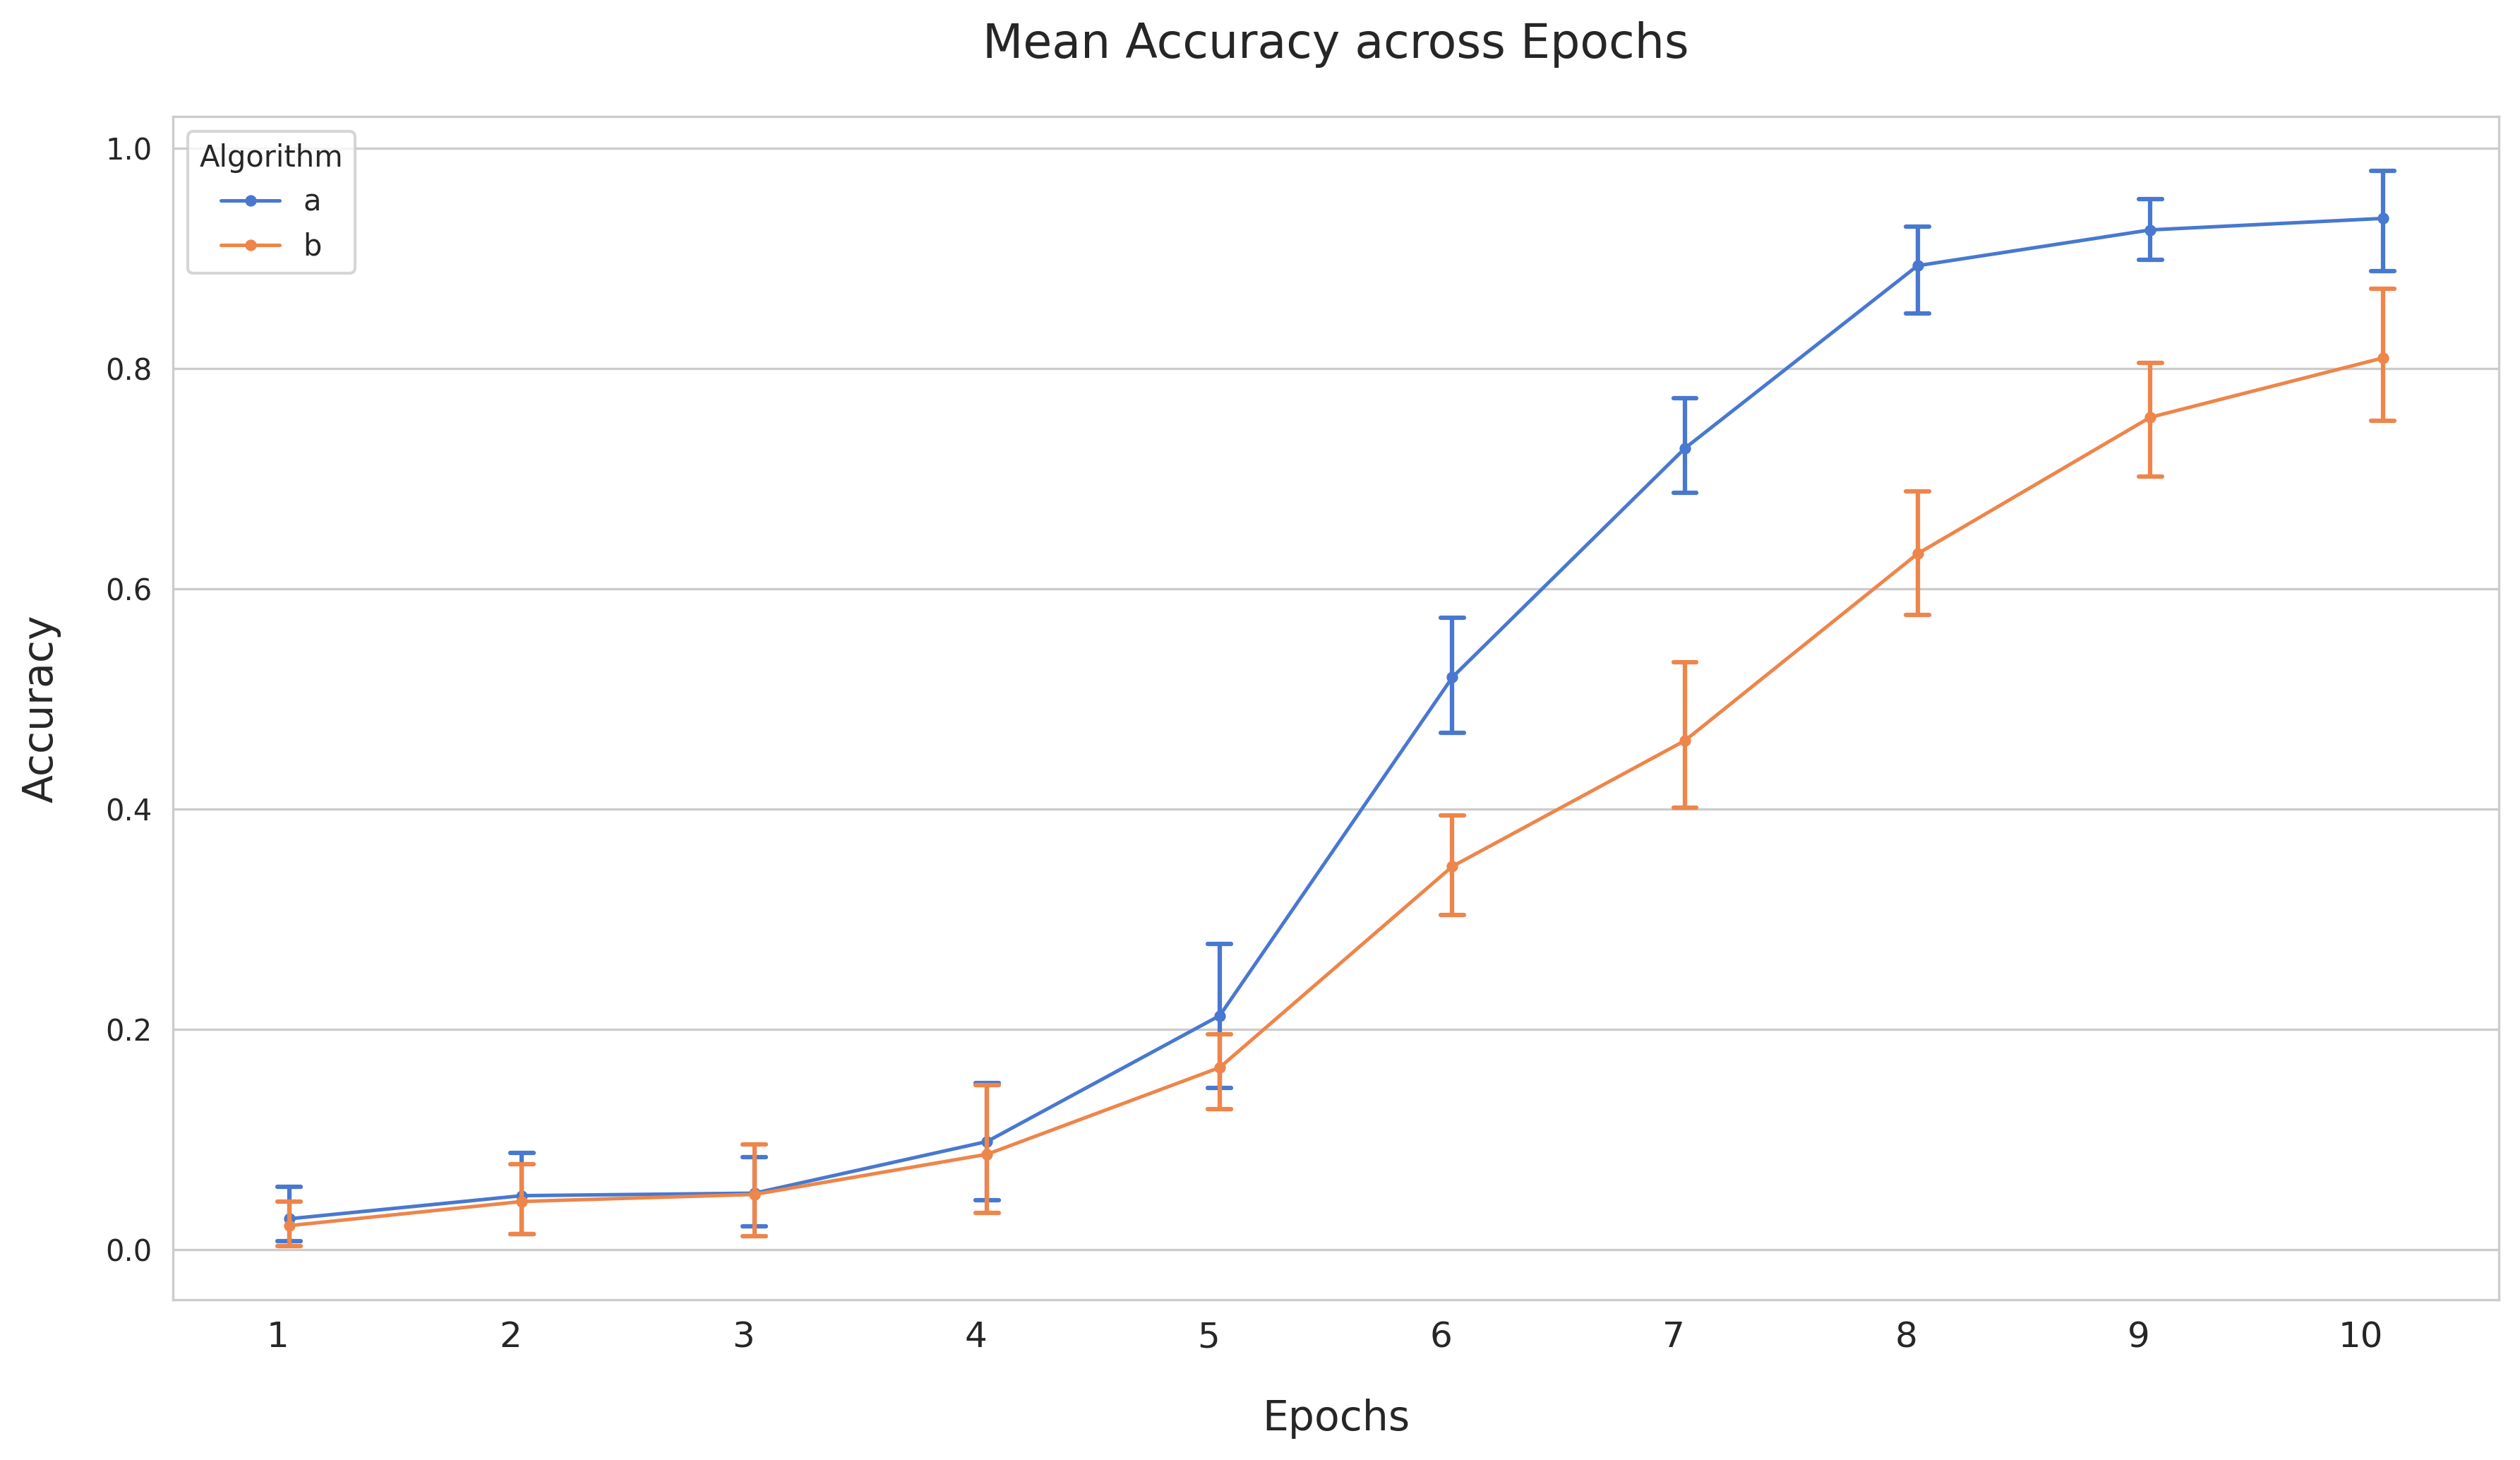
\includegraphics[width=0.95\textwidth]{figures/algo_accuracy_by_epoch_error_bar_plot.png}
  
  \textbf{Figure 13:} Mean Accuracy across Epochs by Algorithm with 95\% confidence intervals.
\end{center}

\textbf{Barcode Chart}
\begin{center}
  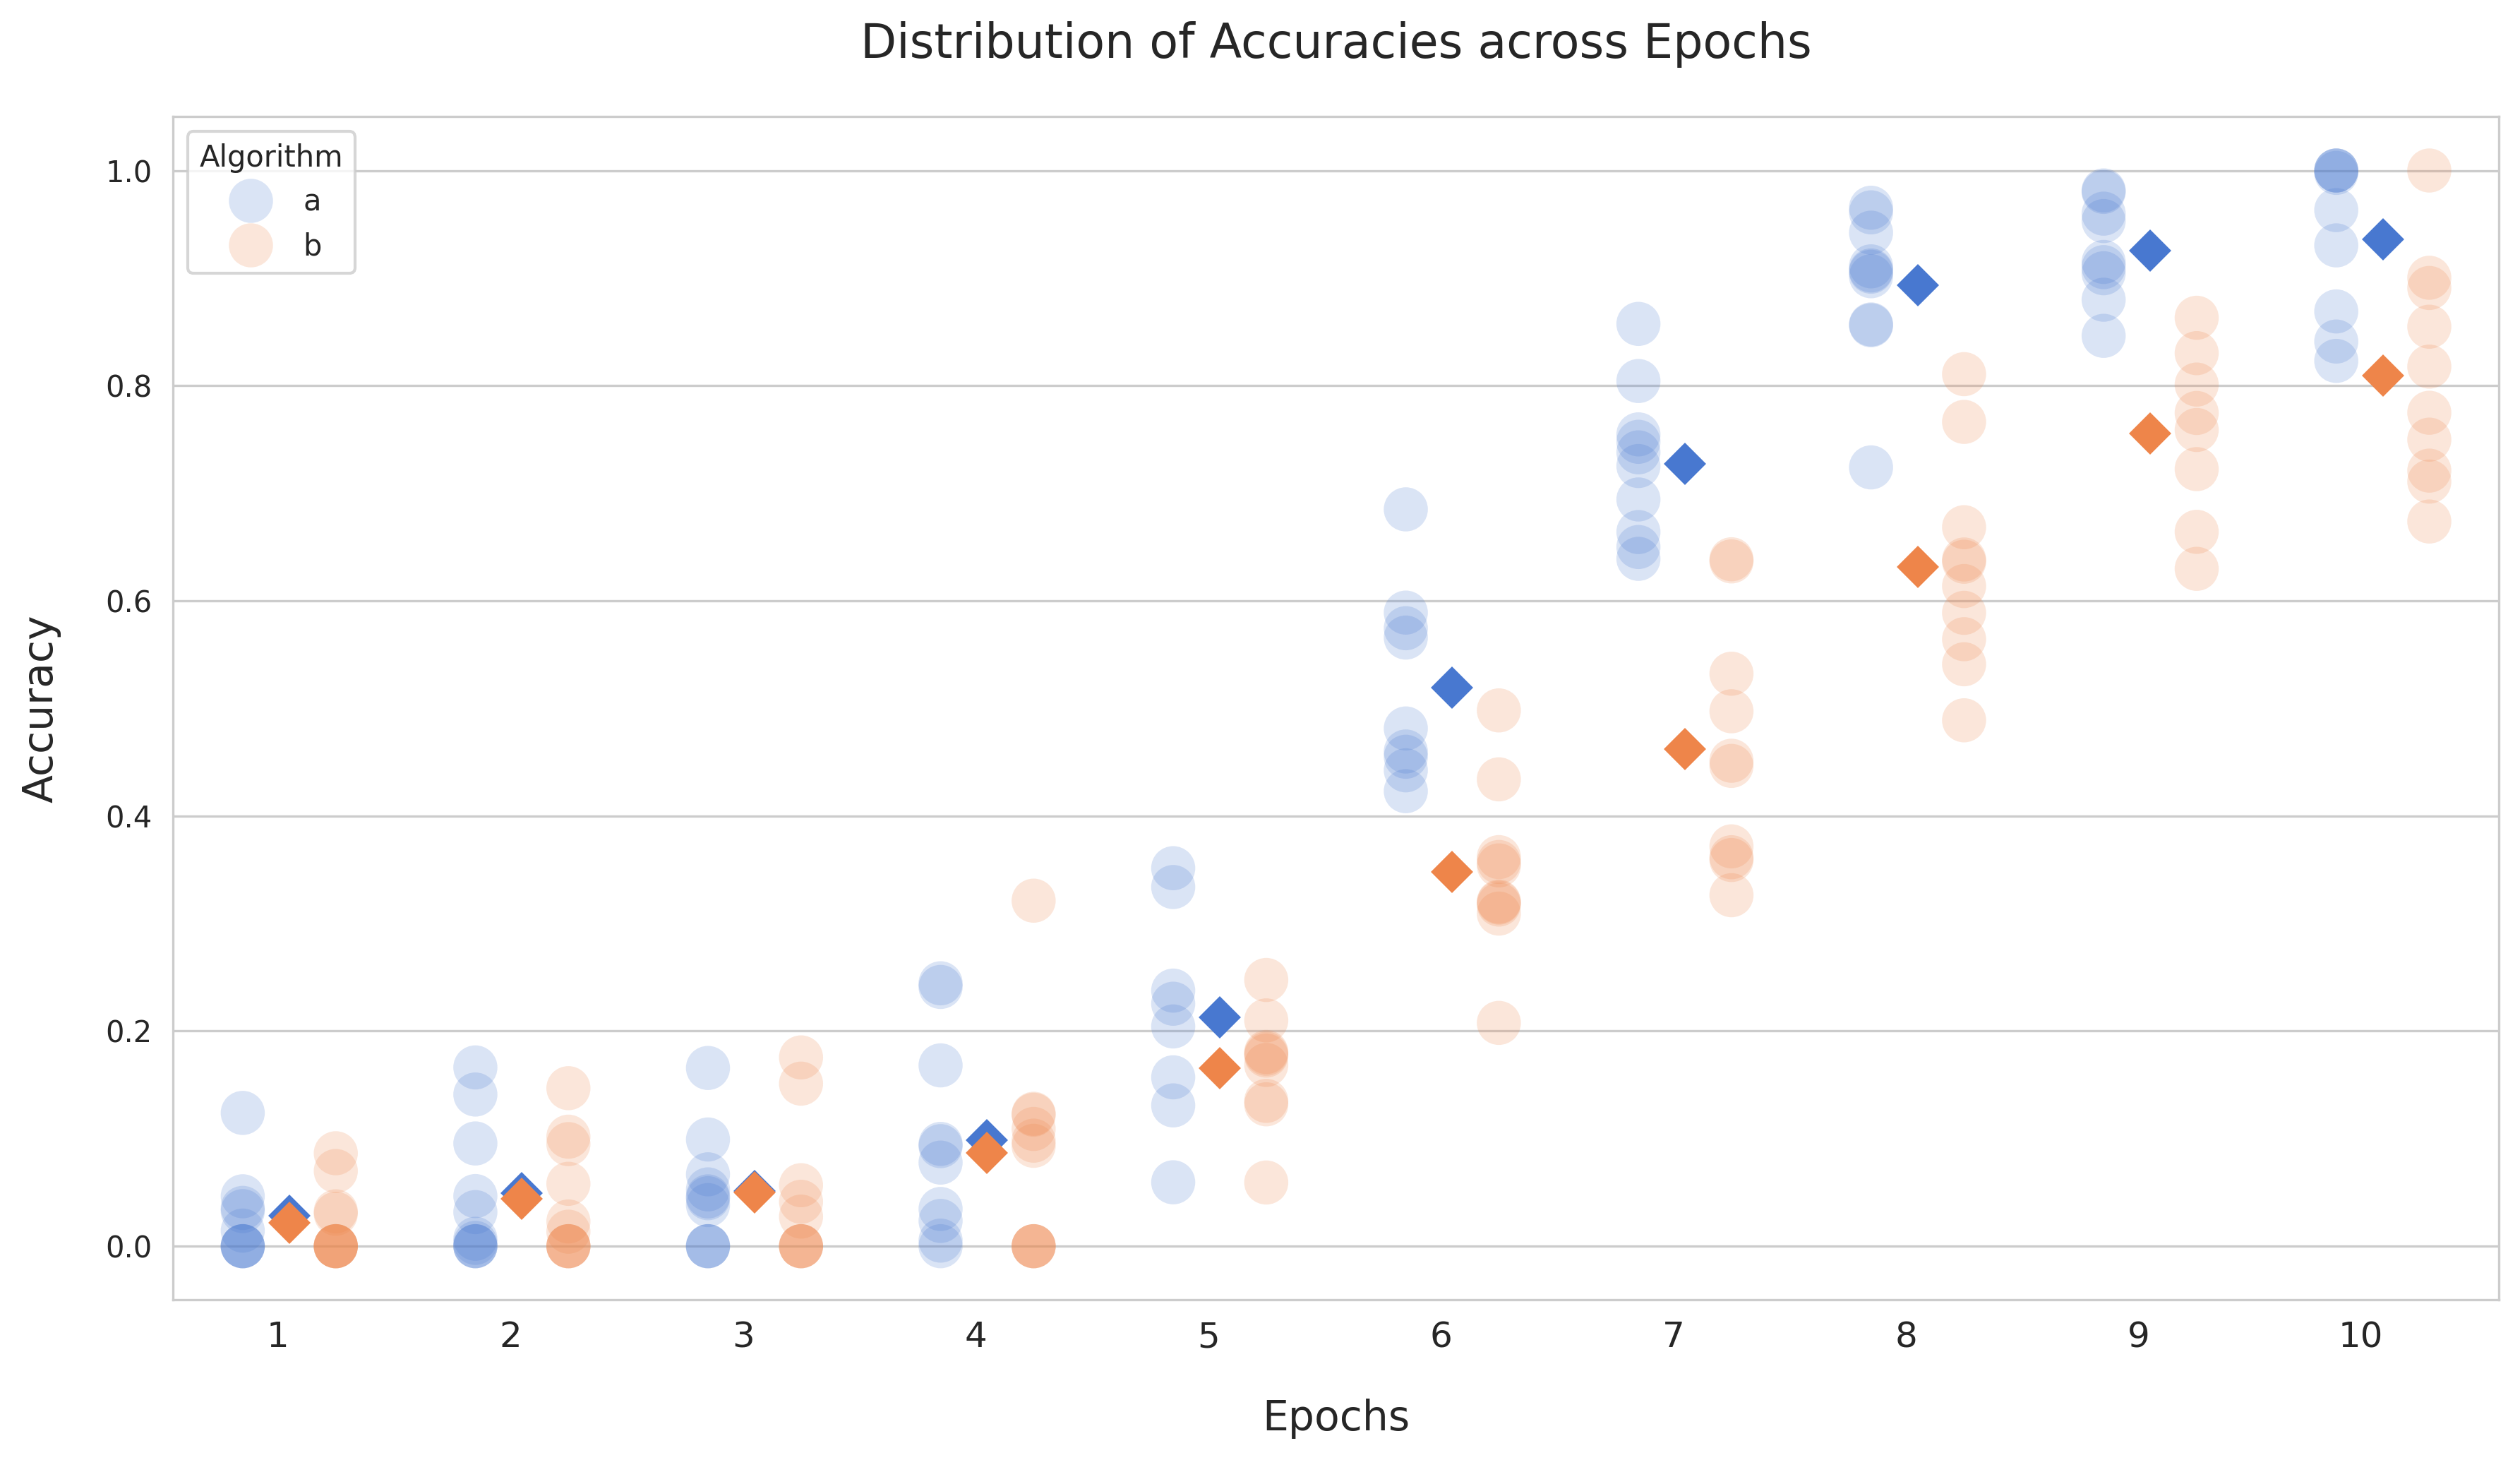
\includegraphics[width=0.95\textwidth]{figures/algo_accuracy_by_epoch_strip_plot.png}
  
  \textbf{Figure 14:} Average Distribution of Accuracy across Epochs by Algorithm.
\end{center}

\textbf{Histogram}
\begin{center}
  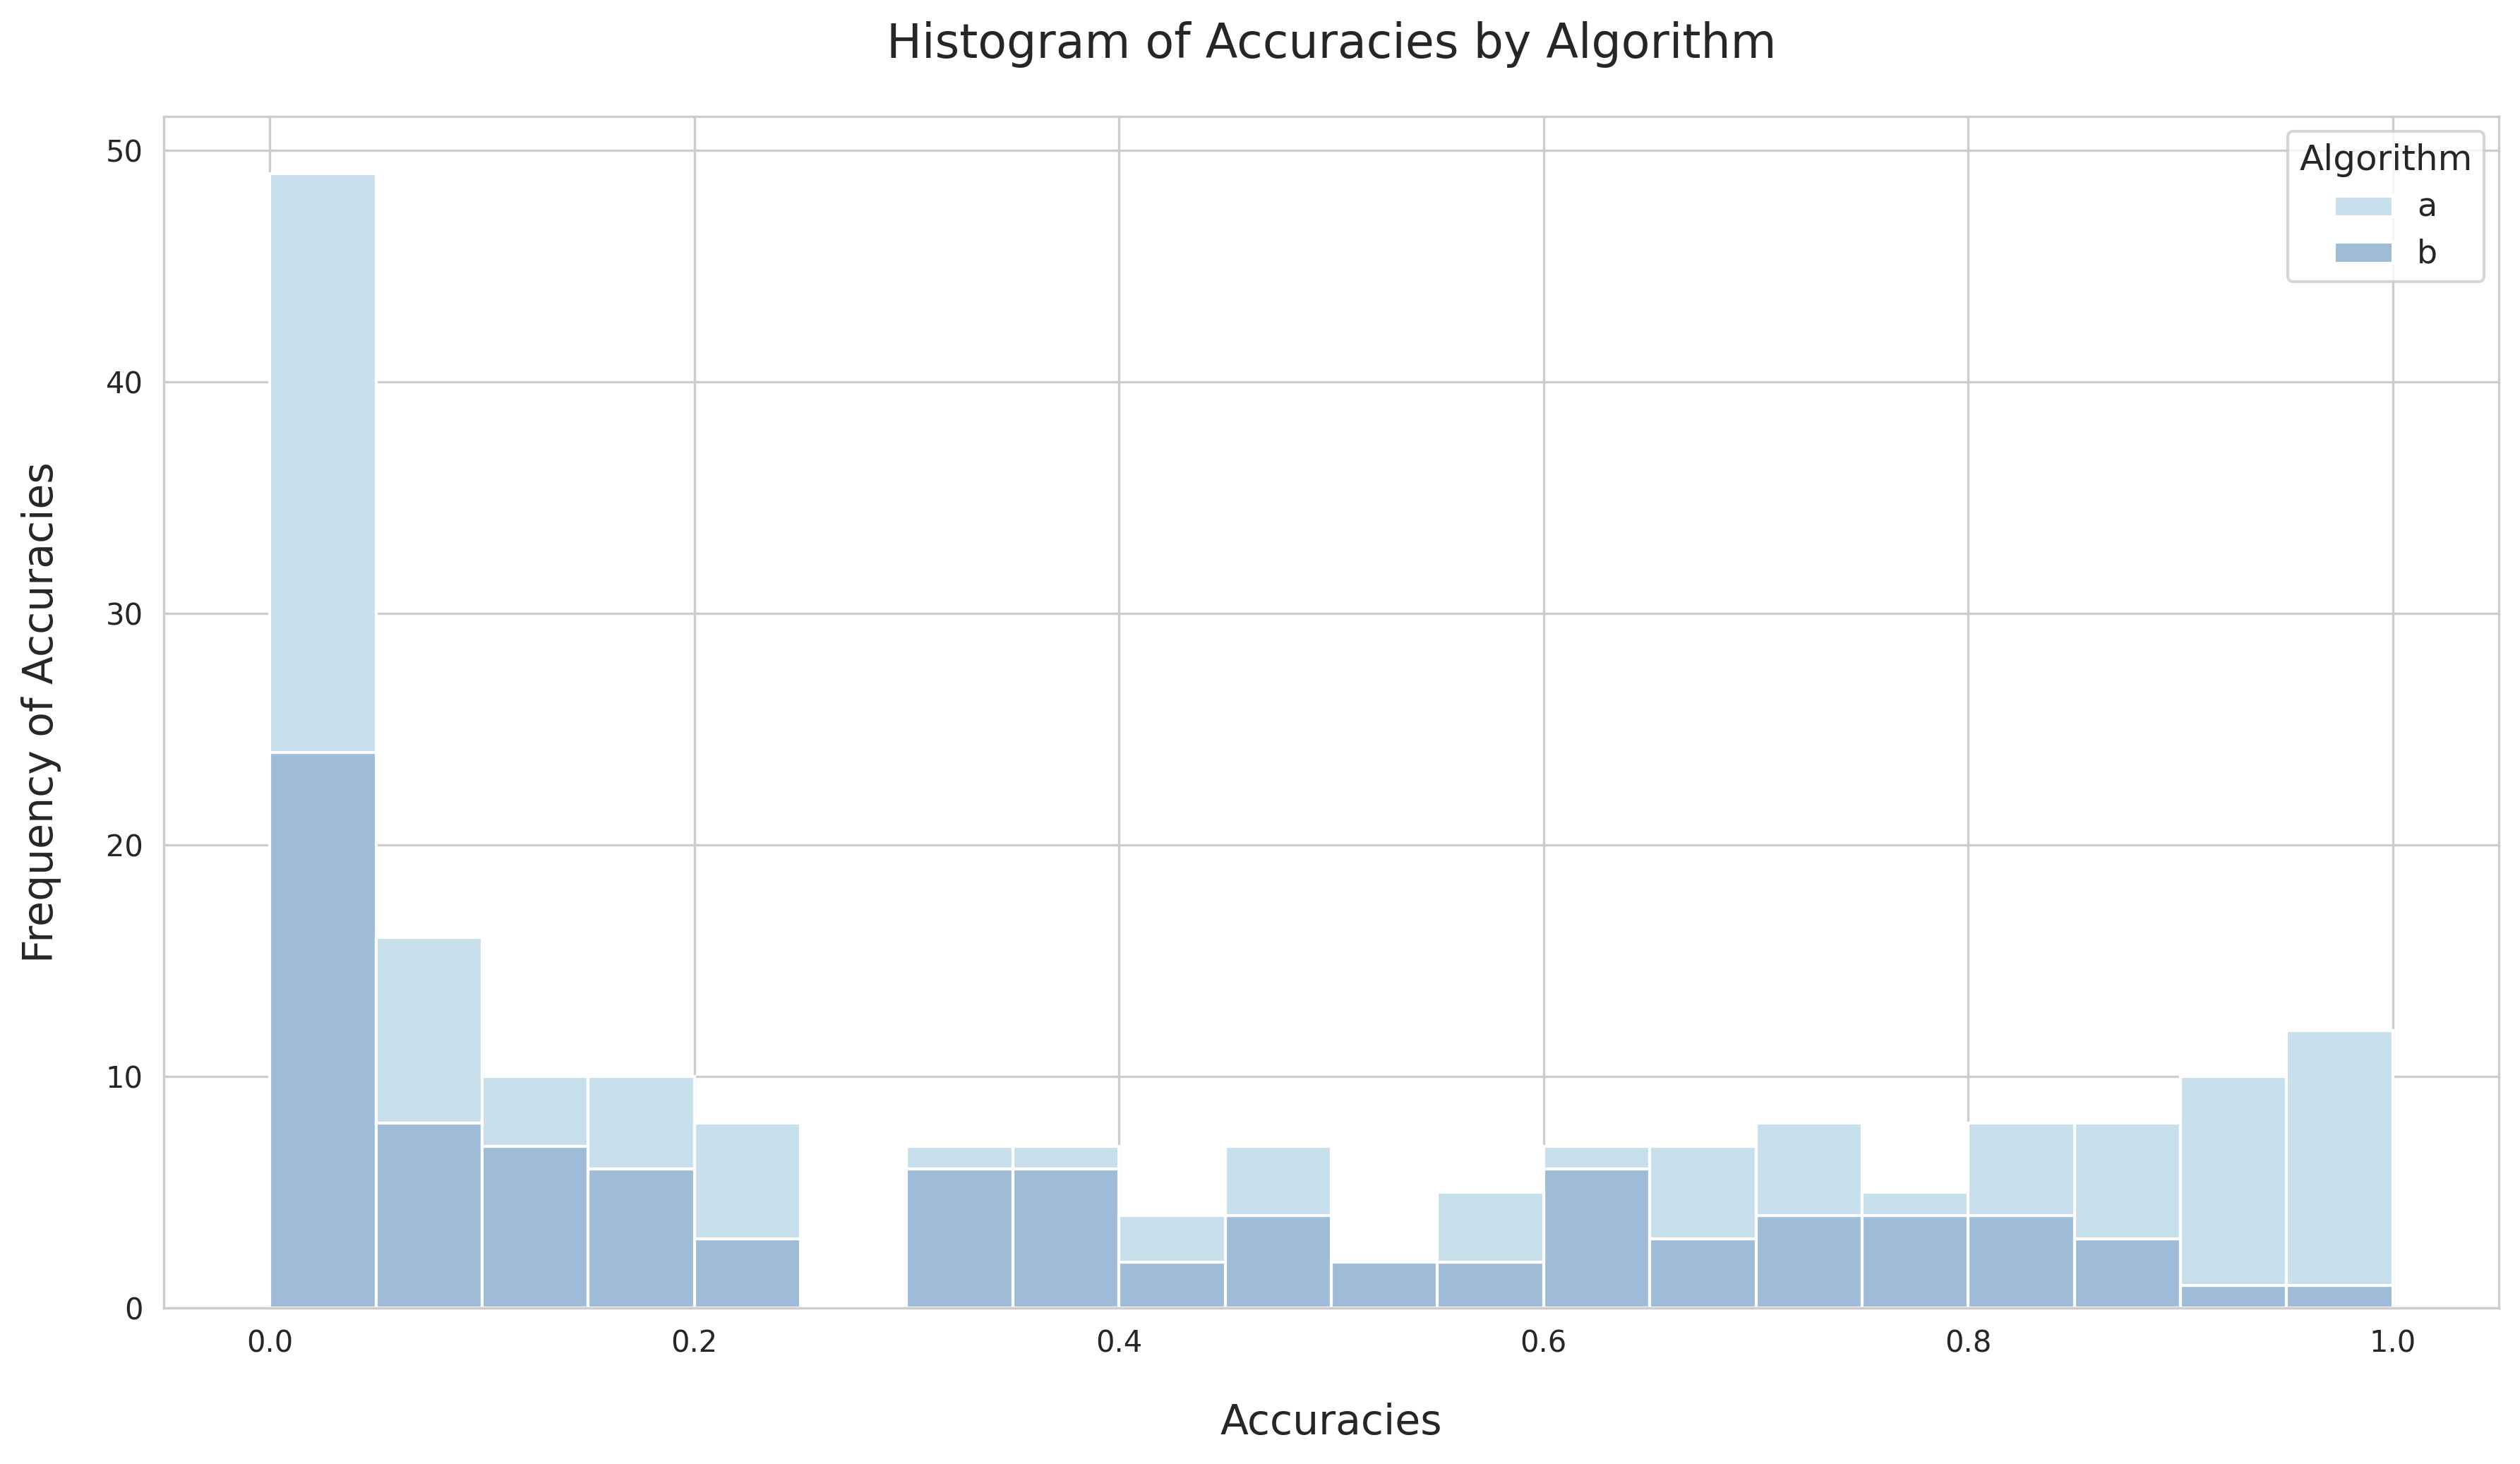
\includegraphics[width=0.95\textwidth]{figures/algo_accuracy_by_epoch_histogram_plot.png}
  
  \textbf{Figure 15:} Histogram of Accuracies by Algorithm.
\end{center}
\newpage

\subsection{Part C: Evaluate and Justify Visualization}
For the dataset:
\begin{itemize}
    \item Discuss the advantages and disadvantages of each visualization type.
    \item Decide which visualization is best for the research question.
    \item Support your answer with evidence from the plots and reasoning based on dataset size, shape, or structure.
\end{itemize}
